\documentclass[aspectratio=169]{beamer}\usetheme{Luebeck} %\usecolortheme{structure}
\definecolor{jred}{HTML}{bd0029}
\definecolor{jblue}{HTML}{0078D7}
\definecolor{primary}{HTML}{00B3B8}
\definecolor{secondary}{HTML}{f39200}
\useoutertheme{infolines}
\setbeamertemplate{page number in head/foot}[framenumber]
\useinnertheme{circles}
\setbeamercolor{palette primary}{bg=primary, fg=white}
\setbeamercolor{palette secondary}{bg=primary, fg=white}
\setbeamercolor{palette tertiary}{bg=primary, fg=white}
\setbeamercolor{palette quaternary}{bg=primary, fg=white}
\setbeamercolor{structure}{fg=primary} % itemize, enumerate, etc
\setbeamercolor{section in toc}{fg=primary} % TOC sections

% Override palette coloring with secondary
\setbeamercolor{subsection in head/foot}{bg=primary!80!white, fg=white}
\usefonttheme{professionalfonts}
\usepackage[utf8]{inputenc}
\usepackage[T1]{fontenc}
\usepackage[english]{babel}
\usepackage{multicol,subcaption}
\usepackage[activate=true, expansion=true, spacing=false]{microtype}
\beamertemplatenavigationsymbolsempty
\usepackage{libertine}
\usepackage{beramono}
\usepackage{minted}
\usepackage{setspace,enumerate}
\usepackage{tikz}
\usetikzlibrary{calc}
\usetikzlibrary{decorations.pathreplacing}

\renewcommand{\UrlFont}{\ttfamily\scriptsize} % smaller link font
\graphicspath{{images}{../images}{../diagrams}}
\def\colorize<#1>{\temporal<#1>{\color{gray!50!white}}{\color{jred}}{\color{black}}}
\newcommand{\btu}{\color{black}\textunderscore}\author{Simon Graber, Julian Z\"oggeler, Maksym Bek}
\date{2026-01-27}
\title{TankGame}
\subtitle{VU Advanced C++ Project}
\titlegraphic{\includegraphics[width=2.5cm]{uibk-color}}

\begin{document}

{
		\usebackgroundtemplate{\includegraphics[width=\paperwidth]{iso3}}
		\begin{frame}\titlepage\small\end{frame}
}

\section{Introduction}
\begin{frame}\frametitle{Agenda - 16 min}
	\begin{itemize}
		\item Overview — 1 min
		\item Structure \& modules — 1 min
		\item Dependencies / tech stack — 1 min
		\item Build / testing / CI — 1 min
		\item Code deep dives — 3 x 3 min
		\item Lessons learned / insights — 1 min
		\item Demo — 3 min
	\end{itemize}
\end{frame}

\begin{frame}\frametitle{Overview (2 min)}
	\begin{itemize}
		\item Multiplayer 2D tank-battle game: menu \textrightarrow\ lobby \textrightarrow\ battle.
		\item Networked gameplay, smooth client experience, fair gameplay.
	\end{itemize}
\begin{figure}
	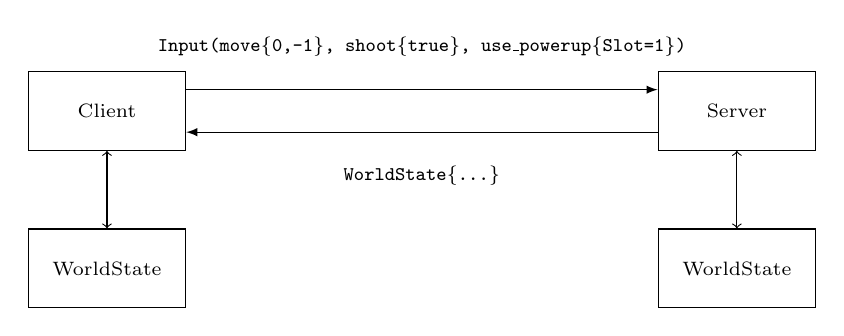
\begin{tikzpicture}[block/.style={draw,minimum width=2cm,minimum height=1cm}, font=\scriptsize]
	\draw (0,0) node[block](C){Client}
	(8,0) node[block] (S) {Server};
	\draw (0,-2) node[block] (CS) {WorldState} (8,-2) node[block] (SS) {WorldState};
	\draw[-latex] (C.15) -- (S.165)
node[midway,above=3mm]{\texttt{Input(move\{0,-1\}, shoot\{true\}, use\_powerup\{Slot=1\})}};
		\draw[-latex] (S.195) -- (C.-15) node[midway,below=3mm]{\texttt{WorldState\{...\}}};
		\draw[<->] (S) -- (SS); \draw[<->] (CS) -- (C);
	\end{tikzpicture}
\end{figure}
\end{frame}

\section{Overview}

\begin{frame}\frametitle{Screenshots}
	\begin{figure}[h]\centering
		\subfloat[Menu]{\includegraphics[width=0.45\textwidth]{menu.png}}\hfill
		\subfloat[Lobby]{\includegraphics[width=0.45\textwidth]{lobby.png}}
	\end{figure}
\end{frame}

\section{Project structure}

\begin{frame}\frametitle{Technical structure — Modules (2.5 min)}\onehalfspacing
	\begin{itemize}
		\item Core: Game loop, States (Menu, Lobby, Battle, ...), Client classes
		\item Network: TCP+UDP, Server-Client, Interpolation system
		\item Game logic: Entities (Players, Projectiles, Items), Map objects
		\item Resources: Templated ResourceManager (textures, fonts, sounds, music)
		\item Tools/tests: CI pipeline for Linux+Windows, headless tests
	\end{itemize}
\end{frame}

\begin{frame}\frametitle{Network Architecture}
	\begin{figure}[h]\captionsetup[subfigure]{labelformat=empty}\centering
		\subfloat[Packet Types]{\includegraphics[width=0.35\textwidth]{TankGame_Utils.pdf}}\hspace{1cm}
		\subfloat[Macro States]{\includegraphics[width=0.55\textwidth]{MacroStates.pdf}}
	\end{figure}
\end{frame}

\begin{frame}\frametitle{Dependencies / Technology stack (1 min)}
	\begin{itemize}\doublespacing
		\item Libraries: SFML, spdlog, Tiled for map assets, nlohmann json parser
		\item CI: Github pipelines: CMake-FetchContent based cross-platform builds
	\end{itemize}
\end{frame}

\begin{frame}\frametitle{Project management}
	\begin{itemize}
		\item Automated tests in CI - litte practical use
		\item Merge Requests to main
		\item Verbose Bugfix commit descriptions
		\begin{itemize}
			\item Previous behaviour
			\item Bug manifestation
			\item Fix description
		\end{itemize}
	\end{itemize}
\end{frame}

\section{Code}
\subsection{Interpolation System (Simon)}

\begin{frame}\frametitle{Interpolation system (3 min)}
	\begin{itemize}\doublespacing
		\item Purpose: hide network latency, smooth gameplay for client
		\item Responsibilities: Predict local movement, interpolate enemies, integrate snapshots
		\item Data Structures: Specialized Ringbuffers holding \emph{ticked} intpus / PlayerState
	\end{itemize}
\end{frame}


\begin{frame}[containsverbatim]
	\frametitle{Data Structures}
	\begin{figure}[h]\doublespacing
		\begin{minted}[fontsize=\small,linenos, style=vs]{cpp}
template<typename T> struct Ticked { uint32_t tick; T obj; };
RingQueue<Ticked<sf::Vector2f>> m_inflightInputs;
RingQueue<Ticked<std::array<PlayerState, 4>>> m_stateBuffer;
         \end{minted}
	\end{figure}
\end{frame}

\begin{frame}{Snapshot interpolation}\centering
	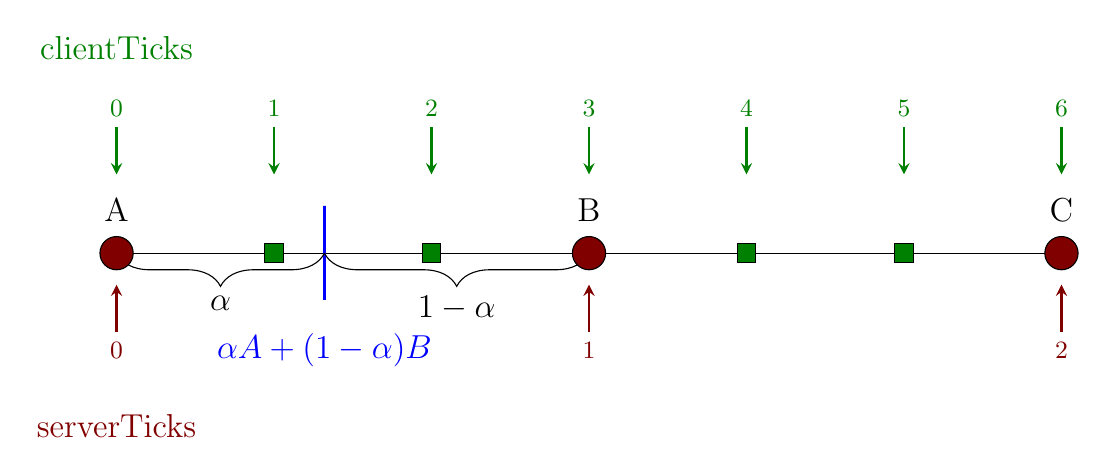
\begin{tikzpicture}[scale=2, every node/.style={font=\large}]

		\coordinate (A) at (0,0);
		\coordinate (B) at (3,0);
		\coordinate (C) at (6,0);
		\draw (A) -- (B) -- (C);
		\def\alphaVal{0.22} %[0,1]
		\coordinate (P) at ($(A)!\alphaVal!(C)$);
		\draw[blue, line width=1pt] (P) -- +(0,.3) -- ++(0,-.3) node[below=8pt] {$\alpha A + (1-\alpha) B$};

		% Curly braces with labels
		\draw[decorate, decoration={brace, amplitude=12pt, mirror}] (A) -- node[below=12pt] {$\alpha$} (P);
		\draw[decorate, decoration={brace, amplitude=12pt, mirror}] (P) -- node[below=12pt] {$1-\alpha$} (B);

		\tikzset{impulse/.style={->, >=stealth, line width=0.8pt}}
		\foreach \i in {0,...,6}{\draw[impulse, green!50!black] (\i,0.8) node[above,font=\small]{\i} -- ++(0,-0.3); \node[rectangle,draw, fill=green!50!black] (r) at (\i,0) {}; }
		\foreach \i in {0,1,...,2}{\draw[impulse, red!50!black] (3*\i,-0.5) node[below,font=\small]{\i} -- ++(0,0.3);}

		\draw[fill=red!50!black] (A) circle (3pt) node[above=8pt]{A}
					(B) circle (3pt) node[above=8pt]{B}
					(C) circle (3pt) node[above=8pt]{C};

		\draw[green!50!black] (0, 1.3) node[anchor=center] {clientTicks};
		\draw[red!50!black] (0, -1.1) node[anchor=center] {serverTicks};
	\end{tikzpicture}
\end{frame}

\subsection{Ammunition Display (Maksym)}


\begin{frame}\frametitle{Ammunition Display (3 min)}
	\begin{itemize}
		\item Purpose: Visual feedback for ammo state and reload progress
		\item Challenge: Smooth animations, intuitive state transitions
		\item Solution: State machine with 4 states per bullet slot
	\end{itemize}
	\begin{figure}[h]\centering
		\includegraphics[width=0.3\textwidth]{reload.png}
	\end{figure}
\end{frame}

\begin{frame}{State Machine Design}\centering
	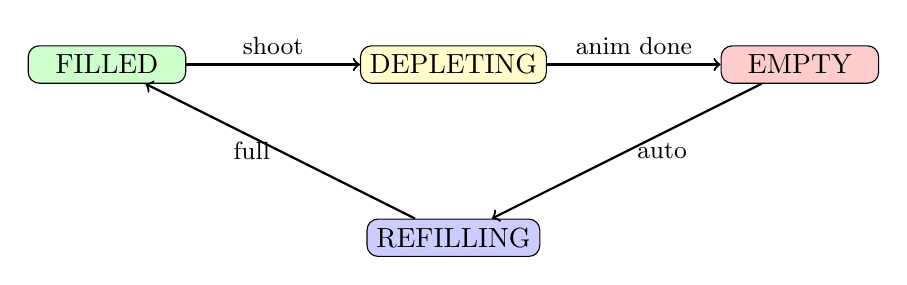
\begin{tikzpicture}[scale=1.1, every node/.style={font=\normalsize}]
		\node[draw, rounded corners, fill=green!20, minimum width=2cm] (F) at (0,0) {FILLED};
		\node[draw, rounded corners, fill=yellow!20, minimum width=2cm] (D) at (4,0) {DEPLETING};
		\node[draw, rounded corners, fill=red!20, minimum width=2cm] (E) at (8,0) {EMPTY};
		\node[draw, rounded corners, fill=blue!20, minimum width=2cm] (R) at (4,-2) {REFILLING};
		\draw[->, thick] (F) -- node[above]{\small shoot} (D);
		\draw[->, thick] (D) -- node[above]{\small anim done} (E);
		\draw[->, thick] (E) -- node[right]{\small auto} (R);
		\draw[->, thick] (R) -- node[left]{\small full} (F);
	\end{tikzpicture}
	\vspace{0.5cm}
	\begin{itemize}
		\item Each bullet slot tracks: \texttt{State} + \texttt{animProgress} $\in [0,1]$
		\item Shooting interrupts reload $\rightarrow$ progress transfers to new slot
	\end{itemize}
\end{frame}

\begin{frame}[containsverbatim]
	\frametitle{Reload Progress Transfer}
	\begin{figure}[h]
		\begin{minted}[fontsize=\scriptsize,linenos, style=vs]{cpp}
void AmmunitionDisplay::onShoot() {
    for (int i = BULLET_COUNT - 1; i >= 0; --i) {
        if (m_bullets[i].state == State::FILLED) {
            m_bullets[i].state = State::DEPLETING;
            m_bullets[i].animProgress = 0.f;

            // Reset any currently reloading bullet to EMPTY
            if (m_currentReloadBullet != -1 && m_currentReloadBullet != i) {
                m_bullets[m_currentReloadBullet].state = State::EMPTY;
                m_bullets[m_currentReloadBullet].animProgress = 0.f;
            }
            // Transfer reload progress to the newly shot bullet
            m_currentReloadBullet = i;
            break;
        }
    }
}
		\end{minted}
	\end{figure}
\end{frame}

\subsection{Connection Monitoring (Julian)}

\begin{frame}[fragile]\frametitle{Heartbeat \& Timeout}
\begin{columns}
\begin{column}{0.5\textwidth}
    \textbf{Client Side (Heartbeat):}
    \begin{itemize}
        \item UDP is connectionless.
        \item If no input is detected, the client sends a \texttt{HEARTBEAT} every 100ms.
        \item Purpose: Maintain presence in the server slot.
    \end{itemize}
\end{column}
\begin{column}{0.5\textwidth}
    \textbf{Server Side (Watchdog):}
    \begin{itemize}
        \item Measures age of the last received packet per slot.
        \item \texttt{elapsed > 5s} $\rightarrow$ Timeout.
        \item Disconnects TCP and clears UDP registration.
    \end{itemize}
\end{column}
\end{columns}

\begin{minted}[fontsize=\tiny, linenos, style=vs]{cpp}
// GameServer::tickStep() - Monitoring & Removal
auto now = std::chrono::steady_clock::now();
for (size_t i = 0; i < m_lobby.m_slots.size(); ++i) {
    if (!m_lobby.m_slots[i].bValid) continue;

    auto elapsed = std::chrono::duration_cast<std::chrono::seconds>(now - m_lastPacketTime[i]).count();
    if (elapsed > 5) {
        SPDLOG_WARN("Client {} timed out", m_lobby.m_slots[i].id);
        m_lobby.removeClient(m_lobby.m_slots[i]); // Invalidate slot & close socket
    }
}
\end{minted}
\end{frame}

\begin{frame}[fragile]\frametitle{Ingame Disconnect Logic}
\textbf{What happens when a player drops?}
\begin{enumerate}
    \item \textbf{Invalidation:} Server marks the slot as \texttt{bValid = false}. (the flag marks the player as connected valid player)
    \item \textbf{Win Condition Check:} The game loop only counts "valid" and "alive" players.
    \item \textbf{Game Over:} If only 1 valid player remains $\rightarrow$ Victory by default.
    \item \textbf{Global Reset:} If 0 players remain $\rightarrow$ \texttt{resetServer()} cleans up.
\end{enumerate}

\begin{minted}[fontsize=\tiny, linenos, style=vs]{cpp}
// GameServer::tickStep() - Determining the winner
size_t cAlive = 0;
PlayerState* lastAlive = nullptr;
for(auto &p : m_world.getPlayers()) {
    // A player only counts if they are alive AND the connection (slot) is still valid
    if(p.isAlive() && m_lobby.m_slots[p.m_id - 1].bValid) {
        cAlive++;
        lastAlive = &p;
    }
}

if(cAlive <= 1) {
    m_winner = lastAlive; // Could be nullptr if everyone disconnected
    return true; // Signals main.cpp that the match has ended
}
\end{minted}
\end{frame}

\begin{frame}[fragile]\frametitle{Fixing \texttt{removeClient}: Ensuring Visual Sync}
The previous version lacked a notification to other clients. To fix the "Ghost Player" issue, we must broadcast the change immediately.

\begin{minted}[fontsize=\tiny, linenos, style=vs]{cpp}
void LobbyServer::removeClient(LobbyPlayer &p) {
    if (p.bValid) {
        // 1. Network Cleanup
        m_multiSock.remove(p.tcpSocket);
        p.tcpSocket.disconnect();

        // 2. Logic Reset
        p.bValid = false;
        p.bReady = false;
        m_cReady = std::max(0, m_cReady - 1);

        // 3. Visual Sync (The Missing Link)
        broadcastLobbyUpdate();
        SPDLOG_LOGGER_INFO(spdlog::get("Server"), "Player {} removed.", p.id);
    }
}
\end{minted}

\textbf{Key Fix:} Adding \texttt{broadcastLobbyUpdate()} ensures that all remaining clients receive a new player list immediately, removing the disconnected player from their screens.
\end{frame}

\begin{frame}[fragile]\frametitle{Server Control \& Resource Management}
\begin{columns}

\begin{column}{0.6\textwidth}
    \textbf{Admin Commands (cmdThread)}
    \begin{itemize}
        \item \textbf{\texttt{quit}}: Initiates a graceful shutdown by setting \texttt{running = false}.
        \item \textbf{\texttt{end}}: Forces the current match to end (\texttt{gameServer->forceEnd()}).
        \item \textbf{\texttt{map [id]}}: Sets the map index for the next round.
    \end{itemize}

    \vspace{0.3cm}
    \textbf{Side Info: Reliable Cleanup (RAII)}
    \begin{itemize}
        \item \textbf{No Memory Leaks:} Destructors automatically close sockets and free memory when \texttt{main()} ends.
        \item \textbf{Safe Shutdown:} \texttt{cmdThread.join()} ensures the admin thread finishes properly.
    \end{itemize}
\end{column}

\begin{column}{0.4\textwidth}
    \begin{minted}[fontsize=\tiny, style=vs]{cpp}
// Command loop logic
while(running) {
    std::string cmd;
    std::getline(std::cin, cmd);

    if(cmd == "quit")
        running = false;
    else if(cmd.rfind("map ", 0) == 0)
        nextMapIndex = std::stoi(cmd.substr(4));
    else if(cmd == "end")
        gameServer->forceEnd();
}
// RAII kicks in after loop:
// 1. Thread joins
// 2. Server objects destroyed
// 3. Sockets closed
    \end{minted}
\end{column}

\end{columns}

\end{frame}

\section{Summary}

\begin{frame}\frametitle{Lessons learned}
	\begin{itemize}
	\item How to use C++ libs in CMake to build a game
	\item Less low-level details than expected
	\item How to use github CI, caching, artifacts, etc.
	\item Application of advanced C++ techniques
	\end{itemize}
\end{frame}

\begin{frame}\frametitle{Demo}
	Playing over VPN with rather bad latency (seen up to 1000ms)
\end{frame}

\end{document}
